\section{Replication Results \& Training Dynamics}
\label{sec:replication_results}

\subsection{Quantitative benchmark results}
Both baseline models were trained from scratch on CIFAR-100 for 100 epochs following the setup in Section~\ref{sec:experimental_setup}. We recorded training loss, training accuracy, validation loss, Top-1 accuracy, and Top-5 accuracy for every epoch into repository logs (\texttt{runs/res\_mlp.log}, \texttt{runs/resmlp.csv}, and \texttt{runs/rep\_mlp.log}).

Table~\ref{tab:quantitative_benchmark} summarizes both training and validation metrics from the 100-epoch benchmark.

\begin{table}[h]
\centering
\adjustbox{max width=\linewidth}{%
\begin{tabular}{llcccccc}
\toprule
\rowcolor{aivnGreen!12}
\textbf{Model} & \textbf{Architecture} & \textbf{Params} & \textbf{Final Train Acc} & \textbf{Epoch 20 Val Acc} & \textbf{Best Val Acc@1} & \textbf{Best Val Acc@5} & \textbf{Train time} \\
\midrule
\textbf{ResMLP} & Isotropic Columnar & 2,191,204 & 44.72\% & 45.52\% & 62.40\% & 87.52\% & 54.65 min \\
\rowcolor{rowLavender!50}
\textbf{RepMLP} & Hierarchical Multi-stage & 2,155,684 & 63.43\% & 55.92\% & 71.46\% & 90.96\% & 107.13 min \\
\bottomrule
\end{tabular}%
}
\vspace{0.6em}
\caption{Benchmark comparison between ResMLP and RepMLP baselines on CIFAR-100 (100 epochs, seed 42).}
\label{tab:quantitative_benchmark}
\end{table}

\begin{figure}[t]
\centering
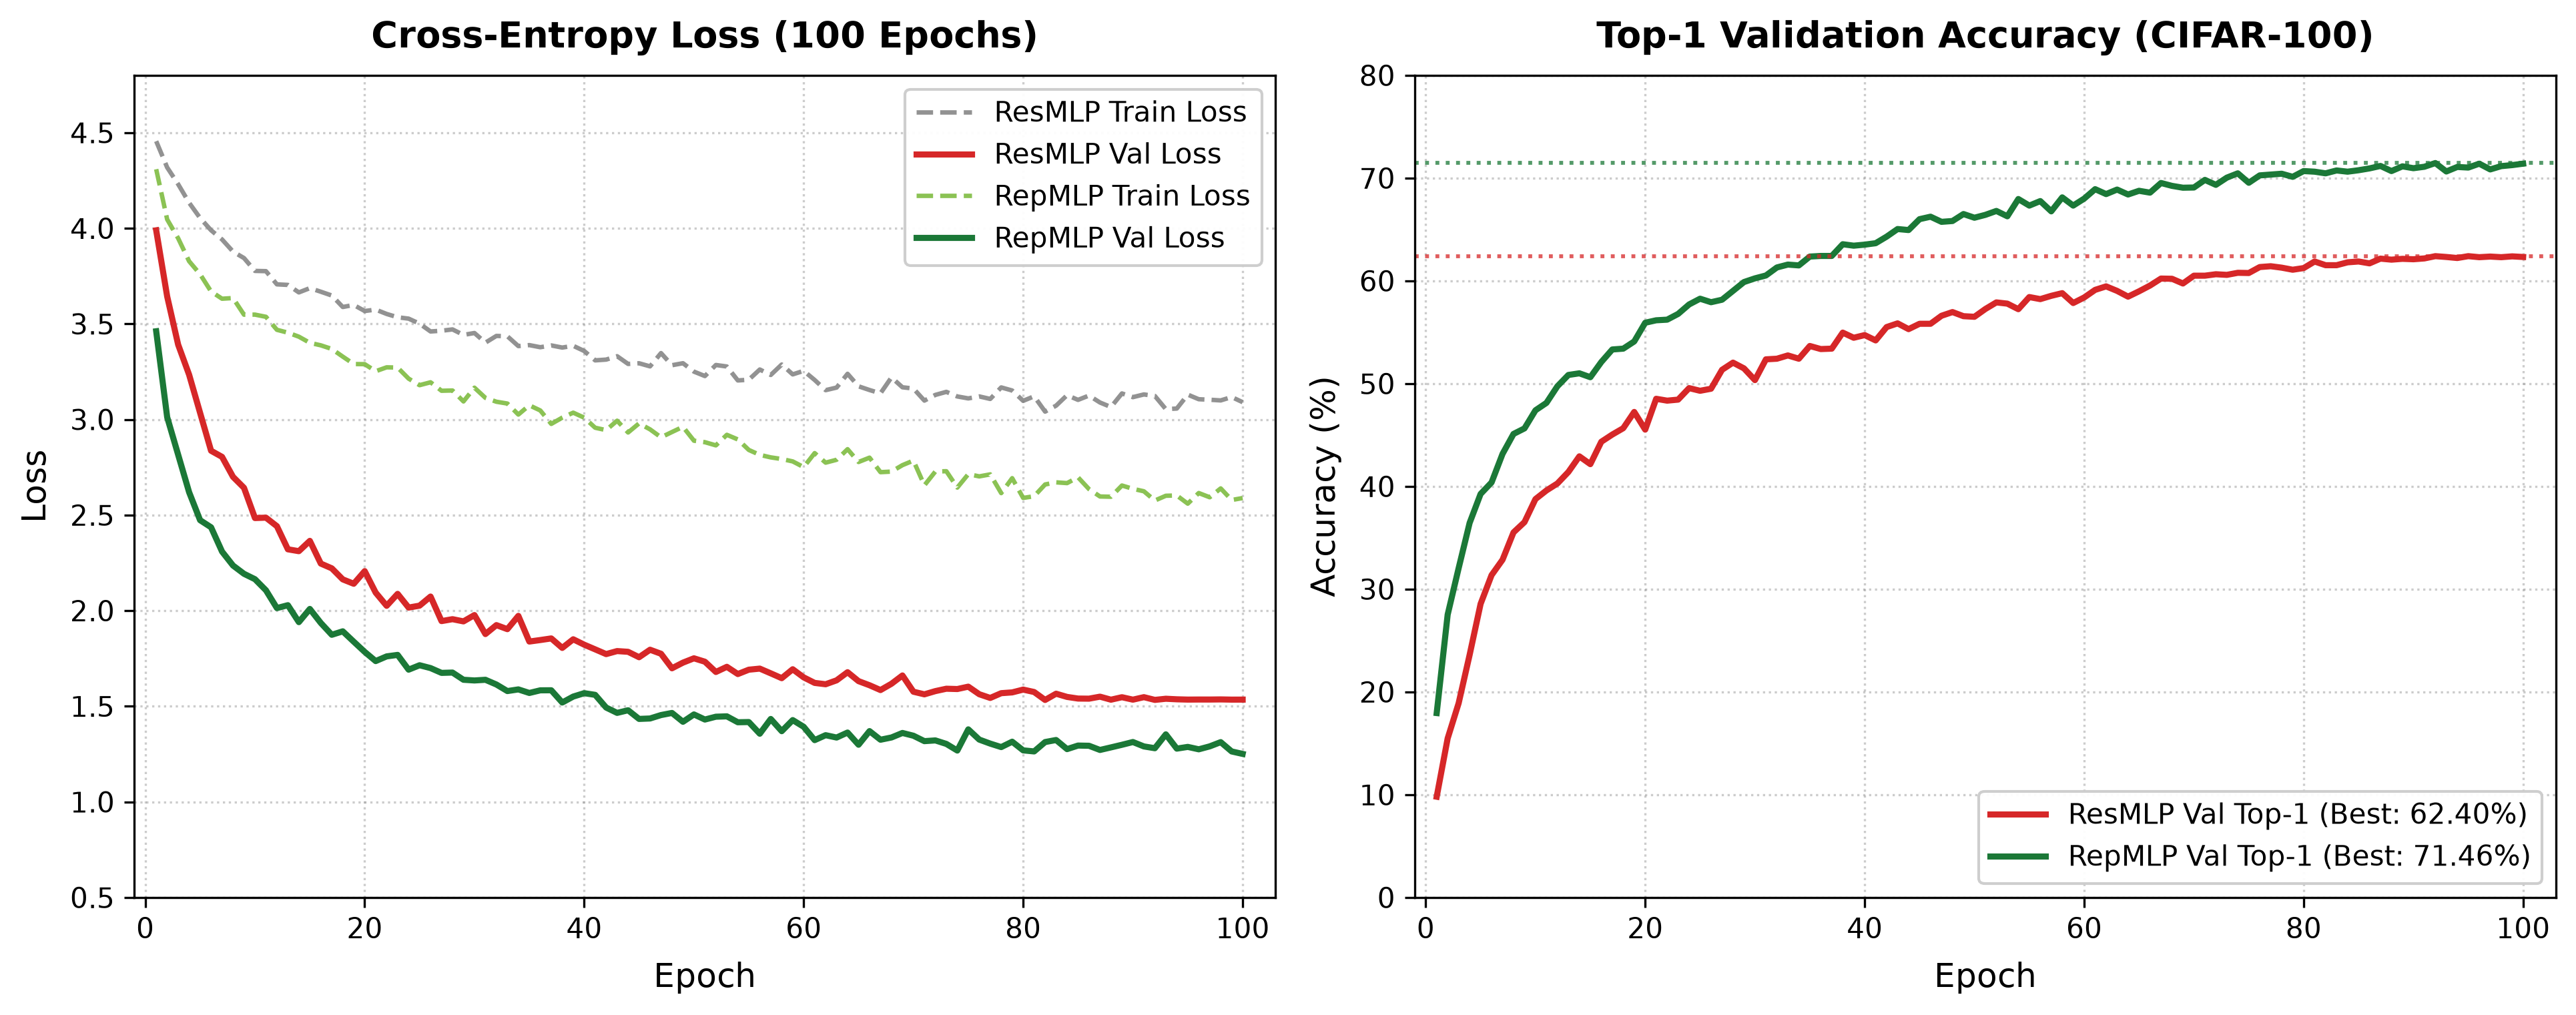
\includegraphics[width=0.95\textwidth]{figures/learning_curves.png}
\caption{Training curves across 100 epochs on CIFAR-100: (Left) Cross-entropy loss on train and validation sets; (Right) Top-1 validation accuracy showing warmup, mid-phase training, and final convergence.}
\label{fig:learning_curves}
\end{figure}

\subsection{Convergence dynamics across 100 epochs}
Looking at both training and validation trajectories across the 100 epochs, we observe three clear phases:

\subsubsection{Phase 1: Early training (epochs 1--20)}
During the first 20 epochs, the two models show very different representation learning speeds on both training and validation splits:
\begin{itemize}[leftmargin=1.5em]
    \item \textbf{RepMLP warms up faster:} At epoch 1, RepMLP starts with train accuracy $7.47\%$ (loss $4.3087$) and validation accuracy $17.94\%$ (loss $3.4612$). By epoch 20, it reaches train accuracy $37.38\%$ (loss $3.2891$) and validation accuracy $55.92\%$ (loss $1.7842$). Its auxiliary $3 * 3$ and $1 * 1$ depthwise conv branches help the model quickly extract low-level spatial features like edges and textures.
    \item \textbf{ResMLP learns spatial relations from scratch:} ResMLP starts slower, with train accuracy $4.53\%$ (loss $4.4553$) and validation accuracy $9.80\%$ (loss $3.9892$) at epoch 1. By epoch 20, it reaches train accuracy $28.47\%$ (loss $3.5670$) and validation accuracy $45.52\%$ (loss $2.2067$), trailing RepMLP by \textbf{$-8.91\%$} in training accuracy and \textbf{$-10.40\%$} in validation accuracy. Because its linear token mixer $\mathbf{W}_{\text{token}} \in \mathbb{R}^{64 \times 64}$ has no built-in notion of 2D locality, it must discover spatial adjacency purely from gradient updates.
\end{itemize}

\subsubsection{Phase 2: Mid-phase training (epochs 20--60)}
Between epochs 20 and 60, both models train under heavy data augmentations (Mixup $\alpha=0.8$, CutMix $\alpha=1.0$, and RandAugment):
\begin{itemize}[leftmargin=1.5em]
    \item \textbf{Impact of data augmentation:} Because Mixup and CutMix blend pairs of images and labels, the training targets are soft and mixed, making training accuracy lower than validation accuracy (evaluated on clean, unmixed images).
    \item \textbf{Loss and accuracy progression:} Both models lower their losses steadily. By epoch 50, RepMLP reaches train accuracy $51.48\%$ (loss $2.8888$) and validation accuracy $66.14\%$ (loss $1.4571$). In comparison, ResMLP reaches train accuracy $39.29\%$ (loss $3.2501$) and validation accuracy $56.50\%$ (loss $1.7507$). RepMLP maintains a consistent advantage of $\approx 12.19\%$ on train accuracy and $\approx 9.64\%$ on validation accuracy.
    \item \textbf{Training stability:} Gradient clipping at maximum norm $1.0$ effectively prevents gradient explosions, ensuring smooth optimization throughout these augmented epochs.
\end{itemize}

\subsubsection{Phase 3: Final convergence (epochs 60--100)}
In the last 40 epochs, the Cosine Annealing schedule smoothly decays the learning rate towards $10^{-6}$:
\begin{itemize}[leftmargin=1.5em]
    \item \textbf{RepMLP peak performance:} At epoch 92, RepMLP reaches its peak validation accuracy of \textbf{71.46\%} (val loss $1.2804$, train acc $62.83\%$), with \textbf{90.96\%} Top-5 accuracy. By epoch 100, it finishes with train accuracy $63.43\%$ (train loss $2.5888$) and validation accuracy $71.40\%$ (val loss $1.2506$).
    \item \textbf{ResMLP peak performance:} ResMLP peaks at \textbf{62.40\%} validation accuracy at epochs 92 and 95 (val loss $1.5331$, train acc $43.96\%$), with \textbf{87.52\%} Top-5 accuracy at epoch 99. By epoch 100, it finishes with train accuracy $44.72\%$ (train loss $3.0903$) and validation accuracy $62.32\%$ (val loss $1.5347$).
    \item \textbf{Comparison of fitting capability:} The final gaps of \textbf{+18.71\%} in train accuracy ($63.43\%$ vs. $44.72\%$) and \textbf{+9.06\%} in validation accuracy ($71.46\%$ vs. $62.40\%$) show that RepMLP is significantly better at fitting complex augmented distributions. This confirms that adding local convolutional priors helps vision models learn much more effectively under data constraints.
\end{itemize}

\subsection{Computational efficiency and training time}
Besides accuracy, our logs record the training runtime for both architectures:
\begin{itemize}[leftmargin=1.5em]
    \item \textbf{ResMLP training speed:} ResMLP completed the full 100 epochs in \textbf{54.65 minutes} ($\approx 32.8$ seconds per epoch) on 2 GPUs. Its columnar structure is simple and fast to run on hardware without tensor reshaping overhead.
    \item \textbf{RepMLP training overhead:} RepMLP required \textbf{107.13 minutes} ($\approx 64.3$ seconds per epoch)---almost double the time of ResMLP. This overhead comes from running multiple parallel conv branches ($1 * 1$ and $3 * 3$ with separate BatchNorm layers) and reshaping partitions at every stage.
\end{itemize}

This comparison highlights a clear trade-off: while RepMLP achieves higher accuracy thanks to local convolutions, its partitioning and multi-branch structure make training significantly slower. This observation motivates our Week 03 plan: designing an isotropic architecture (\textbf{Rep-ResMixer}) that adds re-parameterized convolutions directly into ResMLP's linear token-mixer, aiming to gain the accuracy of convolutions while keeping the high speed of pure MLPs.
